\documentclass[letterpaper,12pt]{article}

\usepackage[margin=1.0in]{geometry}
\usepackage{multirow}
\usepackage{tikz}
\usepackage{amsmath}
\usepackage{hyperref}
\usepackage{standalone}

\usetikzlibrary{shapes.geometric, arrows, fit}

\setlength\parindent{0pt}

\newcommand{\specialcell}[2][c]{\begin{tabular}[#1]{@{}c@{}}#2\end{tabular}}
\newcommand{\xxx}[1]{{\color{red}\bf #1}}
\newcommand{\AxisRotator}[1][rotate=0]{\tikz [x=0.25cm,y=0.60cm,line width=.2ex,-stealth,#1] \draw (0,0) arc (-150:150:1 and 1);}

\begin{document}

\title{\textbf{EE 4388 Senior Design II\\Semester Report}}
\author{Hazen Eckert \hspace{3mm} Omar Hasan \hspace{3mm} Ryan Marcotte \hspace{3mm} Ridhwaan Rahman}
\date{May 11, 2015}
\maketitle

\begin{center}
    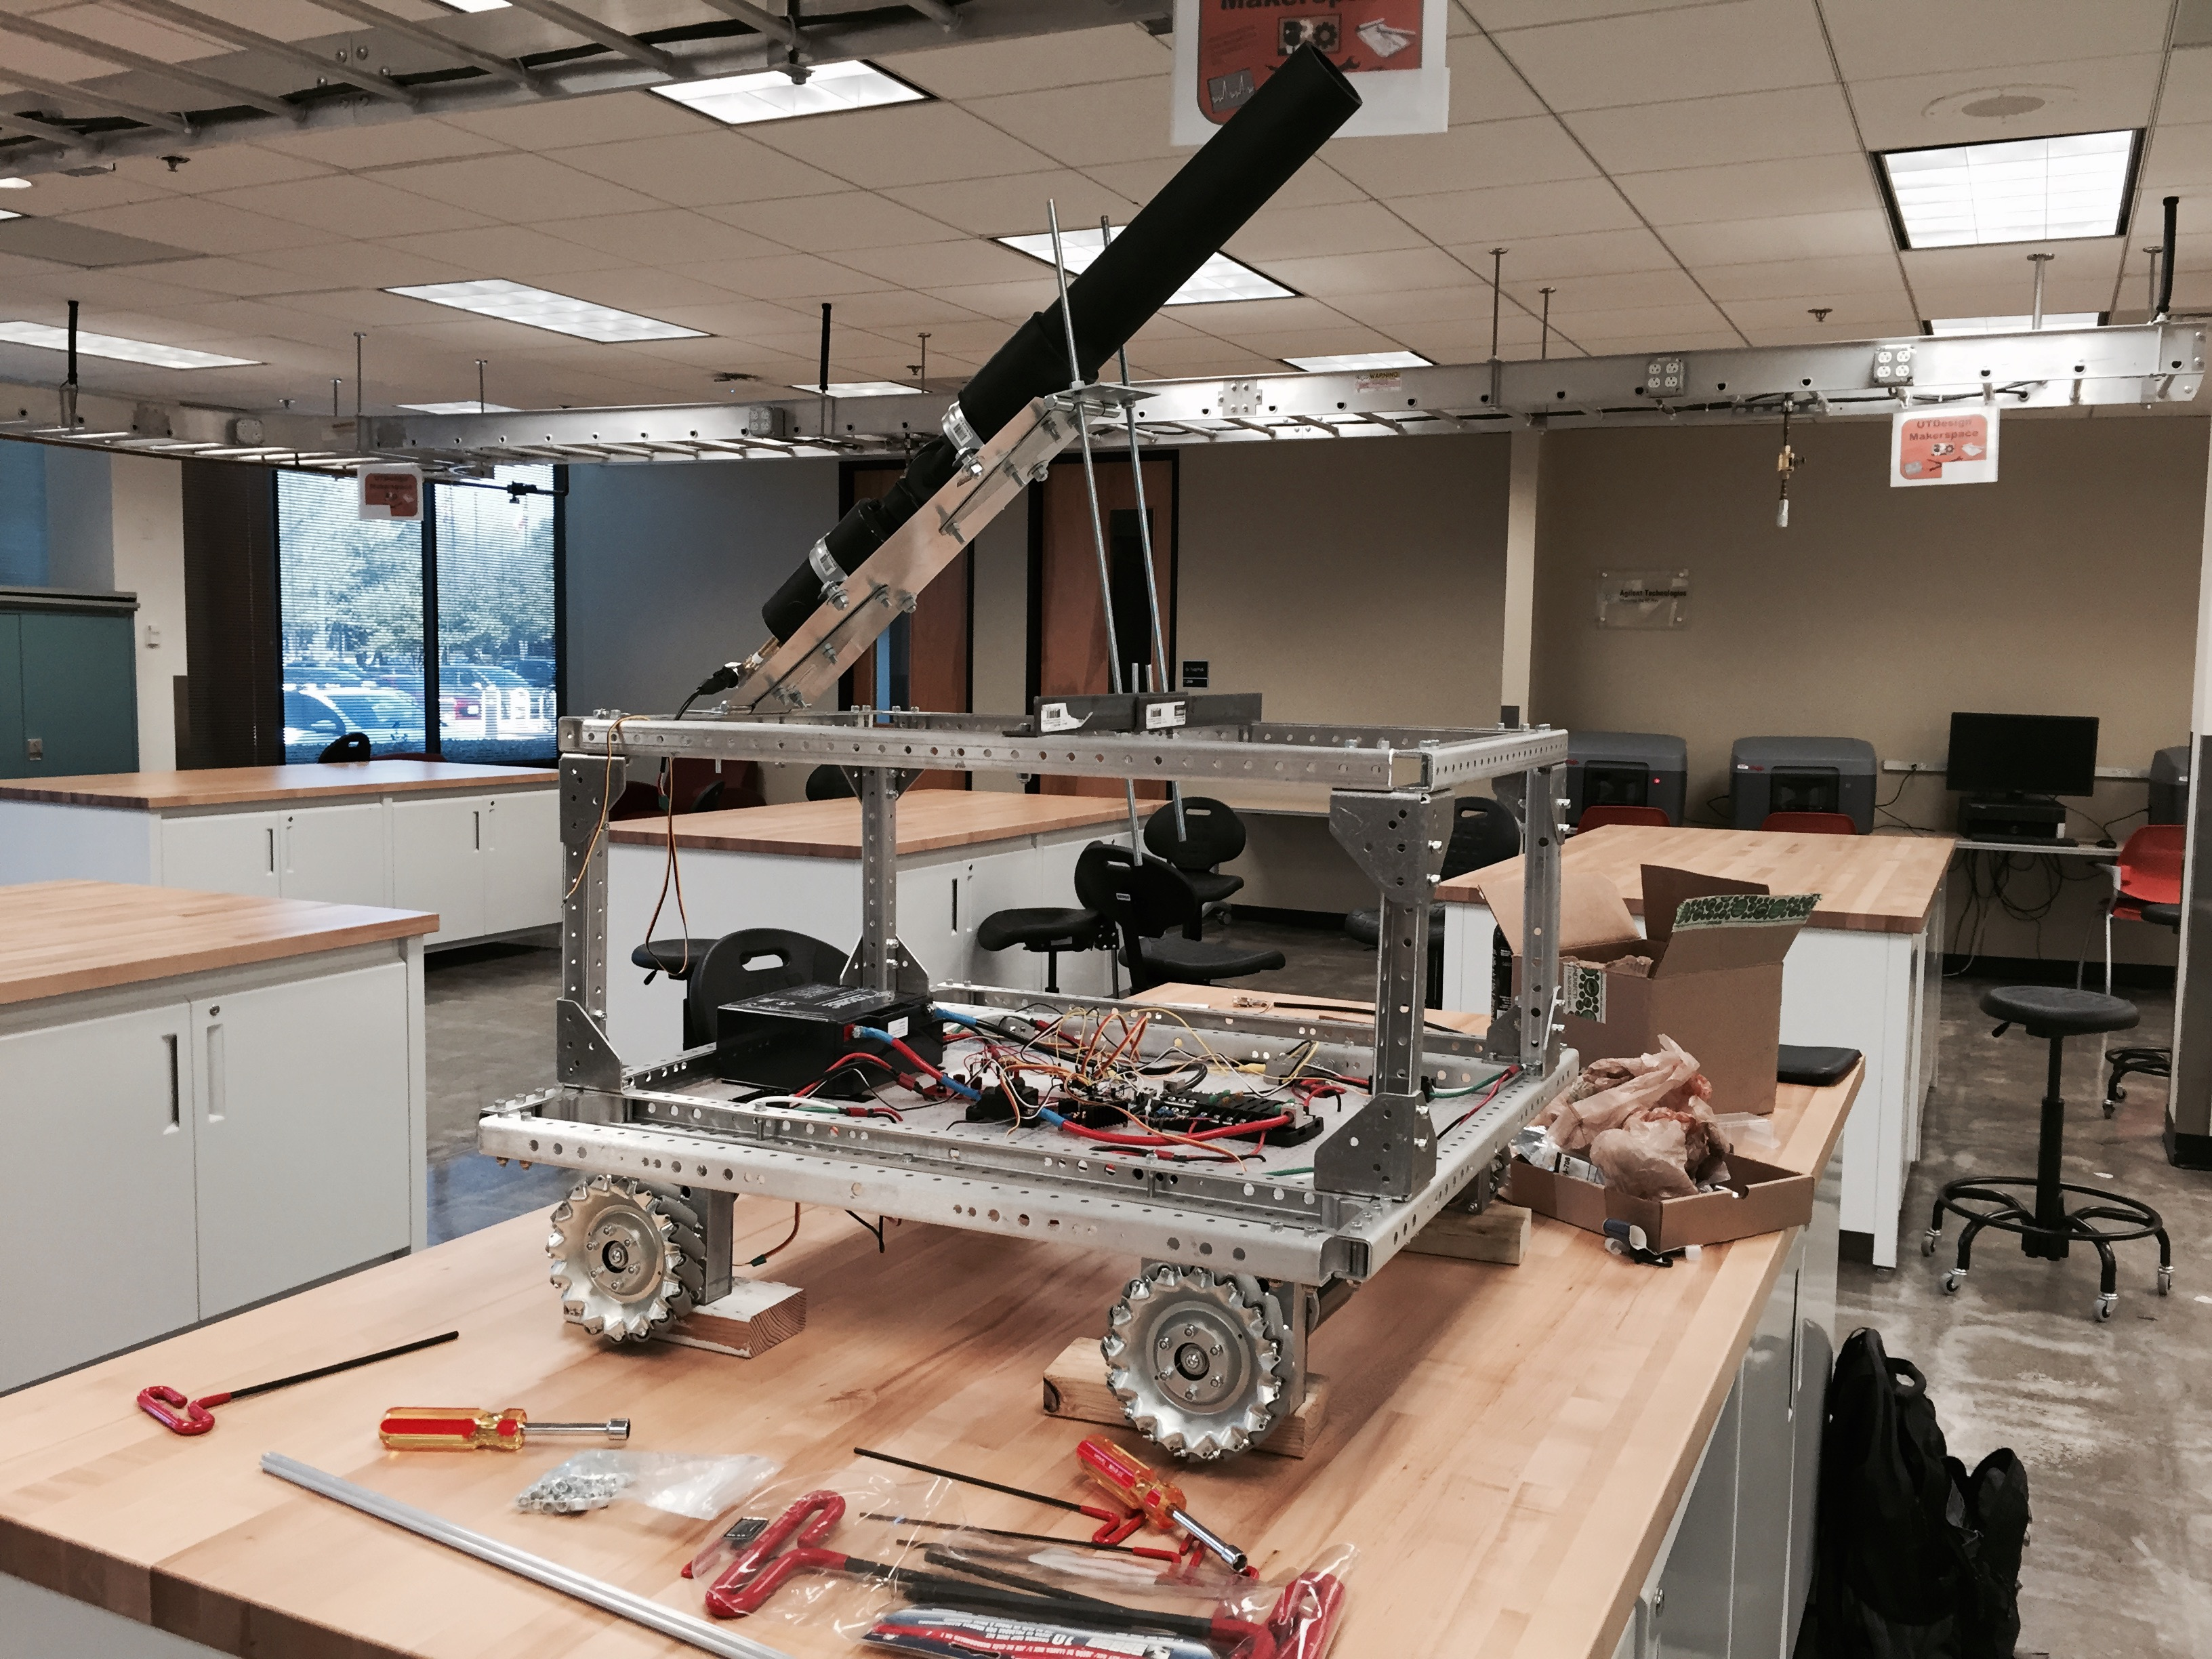
\includegraphics[width=15cm]{./pics/chassis/robot.jpg}
\end{center}

\pagebreak
\tableofcontents
\pagebreak

\section{Introduction}
\label{sec:intro}

\subsection{Purpose}
\label{sec:purpose}
Our task was to design a teleoperated, wheeled mobile robot that can launch
t-shirts safely at university events. The primary purpose of the robot will be
to promote the Erik Jonsson School of Engineering and inspire undergraduate
engineering students to gain hands-on experience with university-sponsored
engineering projects.

\subsection{Problem Statement and Design Objectives}
\label{sec:probstatement}

The design will meet the following objectives:
\begin{itemize}
    \item Operation time \textgreater 10 minutes
    \item Remote control for up to 50 feet
    \item User control of robot velocities and cannon triggering mechanism
    \item Fire t-shirts between 20 and 150 feet
    \item Send live video stream of the robot's First Person View back to the user
\end{itemize}

\subsection{Design Process Summary}
\label{sec:designprocesssummary}
We began designing our robot by determining that the drive system would be
a 4-wheel omnidirectional drive with a t-shirt launching mechanism attached
rigidly to the robot's chassis. Then, a t-shirt launching mechanism was chosen.
An electrical system for wirelessly receiving and transmitting commands and
controlling the robot's movements and t-shirt launching mechanism was designed.
Finally, a software system for handling the robot-user interface was designed.

\subsection{Final Results Summary}
\label{sec:resultssummary}
\xxx{NEED TO DO}

\section{Review of Conceptual and Preliminary Design}
\label{sec:conceptualpreliminarydesign}

\subsection{Problem Analysis}
\label{sec:probanalysis}
The robot must wirelessly receive and perform velocity and t-shirt launching
commands. To perform the commands, the robot must first have a mechanism by
which to control its velocity and also a triggering mechanism for the t-shirt
launcher. The robot must have a wireless receiver on-board and a camera for
first person view streaming. A central controller should coordinate all robot
tasks on-board and a power source for both the t-shirt launching mechanism as
well as the components dedicated to maneuvering the robot. The following
specifications will solve the problem as thus described:

\begin{itemize}
    \item 4-wheel omnidirectional drive
    \item Pneumatic t-shirt launcher with a shot range between 20 and 150 feet
    \item Single power source for all electrical components
    \item Single microcontroller board that includes a microcontroller and
        a microprocessor for embedded linux and wireless communication
    \item Highly reconfigurable IP camera
\end{itemize}

\xxx{Review of problem}\\
\xxx{Summary of specifications}\\
\xxx{Discussion of main features of the design problem}\\
\xxx{Summary of basic engineering or technical approach}

\subsection{Decision Analysis}
\label{sec:decisionanalysis}
We decided for the robot to have 4-wheel omnidirectional drive to allow the
user ease of control over the robot's pose. In this configuration, the user
will be able to separately control the robot's angular velocity and
translational velocity to achieve the desired pose. We chose this configuration
over others because it is simpler to implement and pre-existing solutions are
readily available at certain vendors.\\

The robot's original application is to be used during the halftime of
basketball games to entertain the crowd. Given the size of UTD's basketball
court and bleachers, a shot range between 20 and 150 feet is reasonable for
this application. For convenience, a pneumatic cannon capable of firing single
shots is a widely available commodity that can be retrofitted for our purposes.\\

A single power source would be ideal for powering the robot's 4 motors,
microcontroller, and other electronic devices. We decided to go with a single
power source and use up-conversion and down-conversion voltage regulators
rather than using multiple power sources.\\

A central microcontroller is needed to control the robot's motion and
triggering mechanism. Furthermore, since the robot will need to take wireless
commands as input, it would be ideal to wirelessly program the robot's
microcontroller as well. We chose this solution over using separate
microcontrollers for high and low level commands.\\

\xxx{Description of solution alternatives for the problem}\\
\xxx{Definition of effectiveness criteria}\\
\xxx{Discussion of decision analysis and final decision}

\section{Basic Solution Description}
\label{sec:basicsoldesc}

\subsection{T-Shirt Cannon}
The requirements for our cannon are that it should be electronically
trigger-able, able to shoot a t-shirt 20 to 150 feet from a 45 degree angle,
and be able to make 20 shots on a single charge. The cannon we chose is CO$_2$
based and triggers pneumatically. Other options included a mechanical throwing
mechanism or building the cannon ourselves, but those options would have taken
too much time away from designing the other components. A 20oz CO$_2$ tank
provides enough capacity for at least 20 shots at maximum range. In order to
trigger electronically, we replaced the manual pneumatic trigger with
a solenoid valve. An electronic regulator would not fit within our budget so we
decided to use a pressure transducer and a solenoid valve to allow us to set
the firing pressure of the cannon, and therefore the range, electronically. The
pressure transducer provides the current pressure in the cannon's reservoir and
the solenoid allows us to shut off the flow of CO$_2$ once the desired pressure
is achieved.\\

\subsection{Chassis}
The chassis for our robot has to move holonomically, have maximum speed of 10
ft/s, be safe for gymnasium floors, and have a load capacity of approximately
60 pounds. These requirements led us to choose a four wheeled mecanum drive
system mounted on an aluminum chassis. We chose mecanum wheels because they
have the highest load capacity and simplest control algorithm of the holonomic
drive solutions we could afford. Mecanum wheels have rollers attached at an
angle around the wheel. The wheels can operate like a screw and enable lateral
movement and rotating in place. This comes at the cost of a loss of efficiency
and each wheel requires a separate motor, gearbox, quadrature encoder, and
motor controller.\\

The motors and gearboxes that came with the chassis provide more than enough
torque to achieve 10 ft/s. However, in order to eliminate drift and provide
smoother controls, we decided to include quadrature encoders to provide
velocity feedback for a closed loop control loop. While the motor controllers
we chose can provide 40A continuous current to each motor, our power
distribution system is only capable of delivering 30A to each motor.\\

\subsection{Control Electronics}
An Arduino Yun microcontroller provides the robot with a WiFi
connection and a low level microcontroller. Other options included Texas
Instruments based microcontrollers, but because we wanted simplicity of
programming, we went with the Arduino. The Yun has both an ATmega
microcontroller for low level control as well as an Atheros microprocessor chip
that runs OpenWrt Linux that provides networking capabilities. The Atheros runs
our application that receives velocity, triggering, and other commands over
WiFi and processes them into low level commands for the ATmega. The ATmega
handles hardware interrupt, monitors electrical components, and executes
commands given by the Atheros device. Connected to the ATmega are the motor
controllers, which are controlled via PWM, the quadrature encoder, which sense
rotations of the wheels for velocity feedback, and the pneumatic circuits,
which provide electronic triggering and range adjustment.\\

In the software of the control electronics are several safety power shutoffs.
If communication ceases between the Atheros and the ATmega or between the user
and the Atheros, the robot with shut off the motors. This is achieved through
a “heartbeat“ protocol, which resets a timer every time a message is received.
If no message is received before the timer expires, the connection is assumed
lost and power is shut off.\\

\subsection{User Interface}
The user interface runs on a personal computer running any operating system
with a Java Virtual Machine. An X-Box controller provides the user with
a familiar and intuitive control scheme. The graphical user interface running
on the personal computer updates the user with diagnostic information such as
current firing pressure, battery charge, and connection strength. This
interface also presents the user with a video stream from the robot’s point of
view. A Linux based single board computer, the Raspberry Pi, is streaming this
video from a webcam on the robot.\\

\subsection{Power Distribution System}
The electronic devices on the robot require three different voltages: the
pneumatic components must have 24VDC, the motors need 12VDC, and the control
electronics operate at 5VDC. Since the majority of the current would be drawn
at 12V we chose a 12VDC lead acid battery and used a buck converter to obtain
5VDC and a boost converter to achieve 24VDC. A common automotive fuse box is
used to distribute the 12VDC power among up to 12 circuits at up to 30A. The
battery is able to source up to 300A at any time and can source 60A for 10
minutes straight before discharging. Since our motors will draw at least 2A at
free current, we expect that once the robot achieves a constant velocity, each
motor will draw around 10A. Thus, we expect our battery to give us enough power
to allow the robot to operate for at least 10 minutes at a time.\\

\xxx{In the interest of safety, we have included in the power distribution
system a kill switch that is triggered by physically pulling a bright orange
lanyard.  This cuts the power from the battery to all systems of the robot.}\\

%\noindent Figure \ref{fig:e_system} shows the design of the electrical system.

\xxx{Schematics and flow sheets defining all system components and their relationships}\\
\xxx{Analysis/balance of key parameters (voltage, current, power, timing or computing requirements, mechanical parameters, etc.)}\\
\xxx{Component sizing and component-level specifications}\\
\xxx{Initial system performance estimates}
\begin{figure}[h!]
  \centering

  \tikzstyle{block} = [rectangle, ultra thick, rounded corners, minimum width=3cm, minimum height=2cm,text centered, draw=black]
\tikzstyle{container} = [draw, ultra thick, rectangle, rounded corners, dashed, text width=11em, inner sep=3.5em]
  \tikzstyle{arrow} = [thick, ->, ultra thick, >=latex]
  \begin{tikzpicture}[node distance=2cm]
    \node (input) [align=center, xshift=-1cm] {\textbf{User}\\\textbf{Inputs}};
    \node (output) [right of=input, align=center] {\textbf{Video}\\\textbf{Display}};
    \node (app) [block, yshift=-2cm] {\textbf{Java App}};
    \node (ar9331) [block, right of=app, xshift=6cm, align=center] {\textbf{Atheros AR9331}};
    \node (atmega) [block, below of=ar9331, yshift=-2cm, align=center] {\textbf{ATmega32u4}};
    \node (rpi) [block, below of=app, left of=atmega, xshift=-6cm, yshift=2cm] {\textbf{Raspberry Pi}};

    \node (yun) [container, fit=(atmega) (ar9331)] {};
    \node (yun_text) [yshift=-0.3cm] at (yun.north) {\textbf{Yun}};

    \draw [arrow] (app.350) -- node[anchor=south, align=center, xshift=-7mm, yshift=-11mm] {\textbf{Velocity}\\\textbf{Commands}} (ar9331.190);
    \draw [arrow] (ar9331.170) -- node[anchor=north, align=center, xshift=-7mm, yshift=12mm] {\textbf{Status}\\\textbf{Updates}} (app.10);
    \draw [arrow] (ar9331.250) -- node[anchor=east, align=center] {\textbf{GPIO}\\\textbf{Commands}} (atmega.110);
    \draw [arrow] (atmega.70) -- node[anchor=west, align=center] {\textbf{Sensor}\\\textbf{Readings}} (ar9331.290);
    \draw [arrow] (rpi.70) -- node[anchor=east, align=center, xshift=2cm] {\textbf{Video}\\\textbf{Stream}} (app.290);
    \draw [arrow] (app.250) -- node[anchor=west, align=center, xshift=-2.7cm] {\textbf{Video}\\\textbf{Commands}} (rpi.110);
    \draw [arrow] (input) -- (app.134);
    \draw [arrow] (app.46) -- (output);
  \end{tikzpicture}
  \caption{Software System Diagram}
  \label{fig:system_diagram}
\end{figure}

\begin{figure}[h!]
  \centering
  \tikzstyle{block} = [rectangle, ultra thick, rounded corners, minimum width=2cm, minimum height=1cm,text centered, draw=black]
  \tikzstyle{dcvolt} = [solid, ultra thick, red];
  \tikzstyle{signal} = [solid, ultra thick, ->, >=stealth];

  \begin{tikzpicture}
    draw[help lines] (-6, -12) grid (12,1);
    \node (circuitbreaker) [block, align=center] {\textbf{Circuit}\\\textbf{Breaker}};
    \node (boost) [block, align=center, below of=circuitbreaker, xshift=-4cm, yshift=-2cm] {\textbf{Boost}\\\textbf{Converter}};
    \node (buck) [block, align=center, right of=boost, xshift=7cm] {\textbf{Buck}\\\textbf{Converter}};
    \node (mcu) [block, below of=buck, yshift=-1.25cm] {\textbf{MCU}};
    \node (triggersolenoid) [block, align=center, below of=boost, yshift=-3.5cm, xshift=-1.5cm] {\textbf{Trigger}\\\textbf{Solenoid}};
    \node (pressuresolenoid) [block, align=center, right of=triggersolenoid, xshift=2cm] {\textbf{Pressure}\\\textbf{Solenoid}};
    \node (encoders) [block, right of=pressuresolenoid, xshift=2cm] {\textbf{Encoders}};
    \node (pressuresensor) [block, align=center, right of=encoders, xshift=2cm] {\textbf{Pressure}\\\textbf{Sensor}};
    \node (camera) [block, align=center, right of=pressuresensor, xshift=2cm] {\textbf{Camera}\\\textbf{Module}};
    \node (esc) [block, right of=camera, xshift=2cm] {\textbf{ESC}};
    \node (motors) [block, below of=esc, xshift=-4.5cm, yshift=-1cm] {\textbf{Motors}};

    \draw [dcvolt] (circuitbreaker.north) -- +(0,0.5) node[anchor=south] {\textbf{+12V}};
    \draw [dcvolt] (circuitbreaker.south) -- +(0,-0.9) node[anchor=west, yshift=0.5cm] {\textbf{+12V}};
    \draw [dcvolt] (boost.north) -- +(0,1) -| +(4,1) node {};
    \draw [dcvolt] (buck.north) -- +(0,1) -| +(-4,1) node {};
    \draw [dcvolt] (esc.north) -- +(0,5.55) -| +(-5.5,5.55) node {};
    \draw [dcvolt] (buck.south) -- node[anchor=west, yshift=0.2cm] {\textbf{+5V}} (mcu.north);
    \draw [dcvolt] (encoders.north) -- +(0,2.7) -| +(3.5,2.7) node {};
    \draw [dcvolt] (pressuresensor.north) -- +(0,0.2) -| +(-3,0.2) node {};
    \draw [dcvolt] (camera.north) -- +(0,2.65) -| +(-2.5,2.65) node{};
    \draw [dcvolt] (boost.south) -- +(0,-1) node[anchor=west, yshift=0.5cm] {\textbf{+24V}};
    \draw [dcvolt] (triggersolenoid.north) -- +(0,2.4) -| +(1.5,2.4) node {};
    \draw [dcvolt] (pressuresolenoid.north) -- +(0,2.4) -| +(-1.5,2.4) node {};
    \draw [signal] (pressuresensor.east) -- +(0.5,0) -| +(0.5,0.75) -| +(-0.31, 0.75) -- (mcu.295);
    \draw [signal] (mcu.320) -- +(0,-0.8) -| +(3.5,-0.8) -| +(3.5,-1.75) -- (esc.west);
    \draw [signal] (encoders.east) -- +(0.5,0) -| +(0.5,0.95) -| +(2.39,0.95) -- (mcu.south);
    \draw [signal] (mcu.240) -- +(0,-0.6) -| +(-4.8,-0.6) -| +(-4.8,-1.75) -- (pressuresolenoid.east);
    \draw [signal] (mcu.220) -- +(0,-0.4) -| +(-7.4,-0.4) -| +(-7.4,-1.75) -- (triggersolenoid.east);
    \draw [signal] (esc.south) -- +(0,-1.5) -- (motors.east);
    \draw [signal] (motors.west) -- +(-3.5,0) -| (encoders.south);
  \end{tikzpicture}
  \caption{Electrical System Diagram}
  \label{fig:e_system}
\end{figure}

\section{Performance Optimization and Design of System Components}
\label{sec:optimization}
\xxx{Description of components and their component-level specifications} \\
\xxx{Design criteria used} \\
\xxx{Discussion of the technical approach used} \\
\xxx{Discussion of design details} \\
\xxx{Presentation and discussion of engineering drawings and schematics} \\
\xxx{Fabrication, construction, or production instructions and specifications} \\
\xxx{This section should provide any and all information necessary to ``build'' the component of the design you have focused on, all the way down to the number of nuts, bolts, transistors, wiring harness pin-outs, etc.} \\
\xxx{Summary of the final design results} \\
\xxx{Performance evaluation}

In order to command a desired robot velocity,
\begin{math}
  v=
  \begin{bmatrix}
    v_x \\
    v_y \\
    \omega_z
  \end{bmatrix}
\end{math}
, we calculate the wheel velocities as shown in Equations \ref{eq:rw_to_v}-\ref{eq:v_wheel_4}, according to Figure \ref{fig:robot_top_view}.

\begin{figure}[h!]
  \centering
  \includestandalone[width=\textwidth]{./tikz-figures/kinematics}
  \caption{Top View of Robot}
  \label{fig:robot_top_view}
\end{figure}

\begin{equation}
  v_{wheel}=r_{wheel}\omega_{wheel}
  \label{eq:rw_to_v}
\end{equation}
\begin{equation}
  v_{wheel\,0}=v_x-v_y-(l_1+l_2)\omega_z
  \label{eq:v_wheel_1}
\end{equation}
\begin{equation}
  v_{wheel\,1}=v_x+v_y+(l_1+l_2)\omega_z
  \label{eq:v_wheel_2}
\end{equation}
\begin{equation}
  v_{wheel\,2}=v_x-v_y+(l_1+l_2)\omega_z
  \label{eq:v_wheel_3}
\end{equation}
\begin{equation}
  v_{wheel\,3}=v_x+v_y-(l_1+l_2)\omega_z
  \label{eq:v_wheel_4}
\end{equation}

\begin{table}[h!]
  \centering
  \begin{tabular}{| c | c |}
    \hline
    \textbf{Motor} & \textbf{Position} \\
    \hline
    0 & Forward Left \\
    \hline
    1 & Forward Right \\
    \hline
    2 & Rear Right \\
    \hline
    3 & Rear Left \\
    \hline
  \end{tabular}
  \caption{Motor Numbers}
  \label{tab:motor_nums}
\end{table}

\section{Project Implementation, Operation, and Assessment}
\label{sec:implopassess}
\xxx{Details of implementation} \\
\xxx{Operational test results} \\
\xxx{Evaluation of results relative to design criteria (how well did it do?)} \\
\xxx{What changes are suggested by design results}

\section{Final Scope of Work Statement}
\label{sec:finalscope}

\subsection{T-Shirt Cannon}
The cannon we purchased has been tested manually and can achieve the desired
range of 20 to 150 feet with a capacity of at least 20 shots. The electronic
triggering and pressure regulation components have yet to be assembled and
tested. This will be a priority task for next semester. Once this is completed
we will mount the cannon onto the chassis.\\

\subsection{Chassis, Control Electronics, and Power Distribution System}
The chassis and the power distribution system have been assembled. The control
electronics have been connected to the motors and encoder. The drive system has
yet to be tested due to either defects in the motor controllers or bugs in the
micro controller code. Next semester we hope to fix this issue and test our
maximum velocity. The closed loop control, battery monitoring, and other
software will be implemented next semester.\\

\subsection{User Interface}
\xxx{The current user interface is text based, keyboard controlled, and runs
through a wireless SSH connection to the Atheros chip. We are able to establish
communication between the Atheros and the ATmega and send commands to change
desired motor velocities. Video streaming has been achieved and can be viewed
through the browser on a computer connected to the same network as the
Raspberry Pi. Next semester we will create the user application on a personal
computer and display the video stream through that application’s graphical user
interface. We will write the server application on the Atheros that receives
messages from the user application and implement a full message protocol for
the communication between the Atheros and the ATmega and the user application
and the Atheros.}\\

\xxx{Summarize what has been done} \\
\xxx{Summarize what still needs to be done} \\
\xxx{Lessons learned and suggestions for future activities} \\
\xxx{Describe any special details of the design that only you would know} \\
\xxx{Related project management issues} \\
\xxx{Address complete system life-cycle issues (marketing, sales, service, retirement)}

\section{Cost Estimation}
\label{sec:cost}
1x Arduino Yun MCU: \$65.75 \\
1x Mecanum chassis: \$1012 \\
1x T-shirt cannon: \$365 \\
2x Lead Acid Battery: \$84 \\
1x Electronic Speed Controller: \$45 \\
1x Battery Fuse: \$50 \\
1x Power Converter: \$15 \\
1x Assorted 30A Fuses: \$5.99 \\
1x Power Distribution Board: \$38.69 \\
1x Pi Camera Module: \$26.72 \\
4x Churro Tubes: \$20 \\
4x L Brackets: \$24 \\
1x Raspberry Pi Clear Camera Case: \$8.99 \\
1x CO2 Tank: \$20.99 \\
1x 2-Way 2-pos 1/4in solenoid valve: \$56 \\
1x 150W Boost Converter: \$6.10 \\
1x 200psi Pressure Transducer: \$26 \\
25x 1n4001 diode: \$3.70 \\
10x MOSFET: \$9.14 \\

Miscellaneous (Wire, nuts, bolts, etc): \$15.37 \\

Total Cost: \$1898.44

\xxx{Estimate of system cost (materials and construction)} \\
\xxx{Estimate of design cost (man-hours, materials and supplies, travel)} \\
\xxx{Other (such as construction or production or operating costs)}

\section{Project Management Summary}
\label{sec:projman}

\subsection{Tasks}
Completed:
\begin{itemize}
    \item Pressure sensing and control of the cannon's air tank
    \item Software development on the Arduino Yun
    \item Chassis Assembly
    \item Video streaming
    \item Solenoid as triggering mechanism
\end{itemize}

Future Work:
\begin{itemize}
    \item \xxx{What do we put here?}
\end{itemize}

\subsection{Time}
Two Semesters:
\begin{itemize}
    \item Weekly meetings with Dr. Gans
    \item Weekly meetings among group to organize and assign tasks
    \item \xxx{Why does this section only have two things in it?}
\end{itemize}

\subsection{Budget}
\xxx{Need to fill this out}

\subsection{Facilities}
We conducted our work in the UTDesign Lab in SPN.

\xxx{Tasks: what has been done} \\
\xxx{Tasks: what still needs to be done} \\
\xxx{Time: Gantt chart showing activities and their duration and order} \\
\xxx{Facilities} \\
\xxx{Personnel: summarize personnel needs to complete design; include a WBS}

\section{Conclusion}
\label{sec:conclusion}

\xxx{Restate purpose of report} \\
\xxx{Restate objectives} \\
\xxx{Summarize final design selection} \\
\xxx{Give costs and timeline} \\
\xxx{State willingness to ``keep the customer satisfied''}

\end{document}
